\chapter[Modelado de Requerimientos]{Modelado de Requerimientos}
\label{cp:modelling}

\parindent0pt

El modelo en V es un enfoque de desarrollo de software que enfatiza la importancia de las pruebas en cada fase del ciclo de vida del proyecto. A diferencia del modelo en cascada, donde las pruebas se realizan al final, el modelo en V establece una correspondencia directa entre cada fase de desarrollo (el lado izquierdo de la V) y una fase de pruebas (el lado derecho).

El Modelado de requerimientos es la primera fase en el lado izquierdo de la V. En esta etapa, el objetivo es comprender, documentar y validar las necesidades y expectativas de los interesados en el sistema. Se trata de una fase estratégica antes de comenzar el desarrollo, ya que define lo que el sistema debe hacer y cómo debe comportarse. Un error en esta fase puede tener un efecto dominó en todas las fases siguientes, por lo que dedicar tiempo y esfuerzo para asegurar que los requerimientos sean claros, completos y factibles resulta en un ahorro significativo de tiempo y recursos en las etapas posteriores del proyecto. 

En el contexto de este trabajo de tesis, centrado en el desarrollo de una aplicación basada en tecnología blockchain para la trazabilidad y valorización del vidrio, el modelado de requerimientos fue fundamental para asegurar que el prototipo respondiera a las necesidades específicas de una economía circular transparente y sostenible.

\begin{figure}[!htpb]
    \centering
    
\includegraphics[width=0.6\textwidth]{Figures/requirements-modelling.png}
    \caption{Etapas del proceso de modelado de requerimientos}
    \label{fig:requirements-modelling-process}
\end{figure}

% Revisa la figura inicial: Asegúrate de que la figura requirements-modelling.png sea genérica para el proceso de modelado de requerimientos y no específica de tu proyecto, ya que la describes como las "Etapas del proceso de modelado de requerimientos" en general. Si es una figura propia de tu proceso, considera cambiar la leyenda a "Etapas del proceso de modelado de requerimientos implementado en este trabajo".

La fase de modelado de requerimientos se subdivide a su vez en una serie de pasos estructurados en los cuales los requerimientos se van descubriendo, definiendo y refininando de forma iterativa. En este trabajo de tesis, el modelado de requerimientos comienza con la investigación del dominio del problema para conocer a los actores e interacciones del sistema, con esta información se realiza un Canvas de Propuesta de Valor donde se documentan necesidades y dolencias de cada actor (Sección \ref{sec:domain-definition}). Posteriormente, se realiza un diagrama de casos de uso (Sección \ref{sec:use-cases}) para pasar a la definición de requerimientos funcionales y no funcionales junto con sus interdependencias (Sección \ref{sec:requirements-definition}). Finalmente, se escriben las historias de usuario a partir de la lista de requerimientos, donde se definen los criterios de aceptación de cada requerimiento desde el punto de vista de un usuario del sistema (Sección \ref{sec:user-stories}). Las historias de usuario tienen un nivel de granularidad suficiente como para comenzar las etapas de diseño de arquitectura, estimación de esfuerzo y planificación de la generación de código.


(((

En esta primera etapa de la tesis, se adoptó el **modelo en V** como marco metodológico para el desarrollo del software. Este enfoque, a diferencia del modelo en cascada, enfatiza la integración de las pruebas a lo largo de todo el ciclo de vida del proyecto. Su estructura establece una correspondencia directa entre cada fase de desarrollo, ubicada en el lado izquierdo de la 'V', y una fase de validación y verificación en el lado derecho.

---

### **Modelado de Requerimientos en el Modelo en V**

El **modelado de requerimientos** constituye la fase inicial en el lado izquierdo del modelo en V. El objetivo principal de esta etapa es comprender, documentar y validar las necesidades y expectativas de los interesados del sistema. Dada su naturaleza estratégica, esta fase es crucial para definir de forma precisa el comportamiento y las funcionalidades del sistema. Errores o ambigüedades en esta etapa pueden generar un efecto dominó en las subsiguientes fases de diseño, implementación y pruebas, resultando en un incremento de costos y tiempo. Por ello, la inversión de esfuerzo para asegurar que los requerimientos sean claros, completos y factibles es fundamental para el éxito del proyecto.

En el contexto de este trabajo, centrado en el desarrollo de un prototipo de aplicación con tecnología blockchain para la trazabilidad y valorización del vidrio, el modelado de requerimientos se ejecutó de forma rigurosa para garantizar que el sistema respondiera a las necesidades específicas de una economía circular sostenible y transparente.

El proceso de modelado de requerimientos se estructuró en una serie de pasos iterativos para descubrir, definir y refinar los requisitos. Este proceso se resume en la Figura \ref{fig:requirements-modelling-process}.

\begin{figure}[!htpb]
    \centering
    
\includegraphics[width=0.6\textwidth]{Figures/requirements-modelling.png}
    \caption{Etapas del proceso de modelado de requerimientos}
    \label{fig:requirements-modelling-process}
\end{figure}

El proceso dio inicio con una investigación exhaustiva del dominio del problema para identificar los actores clave y sus interacciones. A partir de esta información, se elaboró un **Canvas de Propuesta de Valor** para documentar de manera flexible las necesidades y problemáticas de cada actor. Posteriormente, se modelaron los **casos de uso** para describir las funcionalidades del sistema desde la perspectiva del usuario. Esto sirvió como base para la definición formal de los **requerimientos funcionales y no funcionales**, incluyendo sus interdependencias. Finalmente, se redactaron **historias de usuario** con un nivel de detalle suficiente para definir los criterios de aceptación, lo cual permitió iniciar las etapas de diseño de arquitectura, estimación de esfuerzo y planificación de la implementación.

)))
\section{Definición de Dominio}
\label{sec:domain-definition}

% TODO: acá traer a colación el título de la tesis y el objetivo de la misma, que es la trazabilidad del vidrio y su valorización. Por ejemplo: garantizar una trazabilidad transparente y la valorización del vidrio.

El primer paso en el modelado de requerimientos es la definición del dominio del problema. En este contexto, se busca comprender el entorno en el que se desarrollará el sistema de trazabilidad de vidrio, identificando los actores clave y sus interacciones con el sistema. Este análisis permite establecer una base sólida sobre la cual se construirán los requerimientos del sistema.

La definición del dominio se realiza a partir de la investigación y revisión de literatura relacionada con la trazabilidad del vidrio. Se examinan las etapas del ciclo de vida del vidrio, desde su producción hasta su reciclaje, identificando los puntos críticos donde la trazabilidad con blockchain puede aportar valor. En la Figura \ref{fig:domain-model} se presenta un diagrama que ilustra las etapas del ciclo de vida del vidrio y los actores involucrados en cada una de ellas.

\begin{figure}[!htpb]
    \centering
    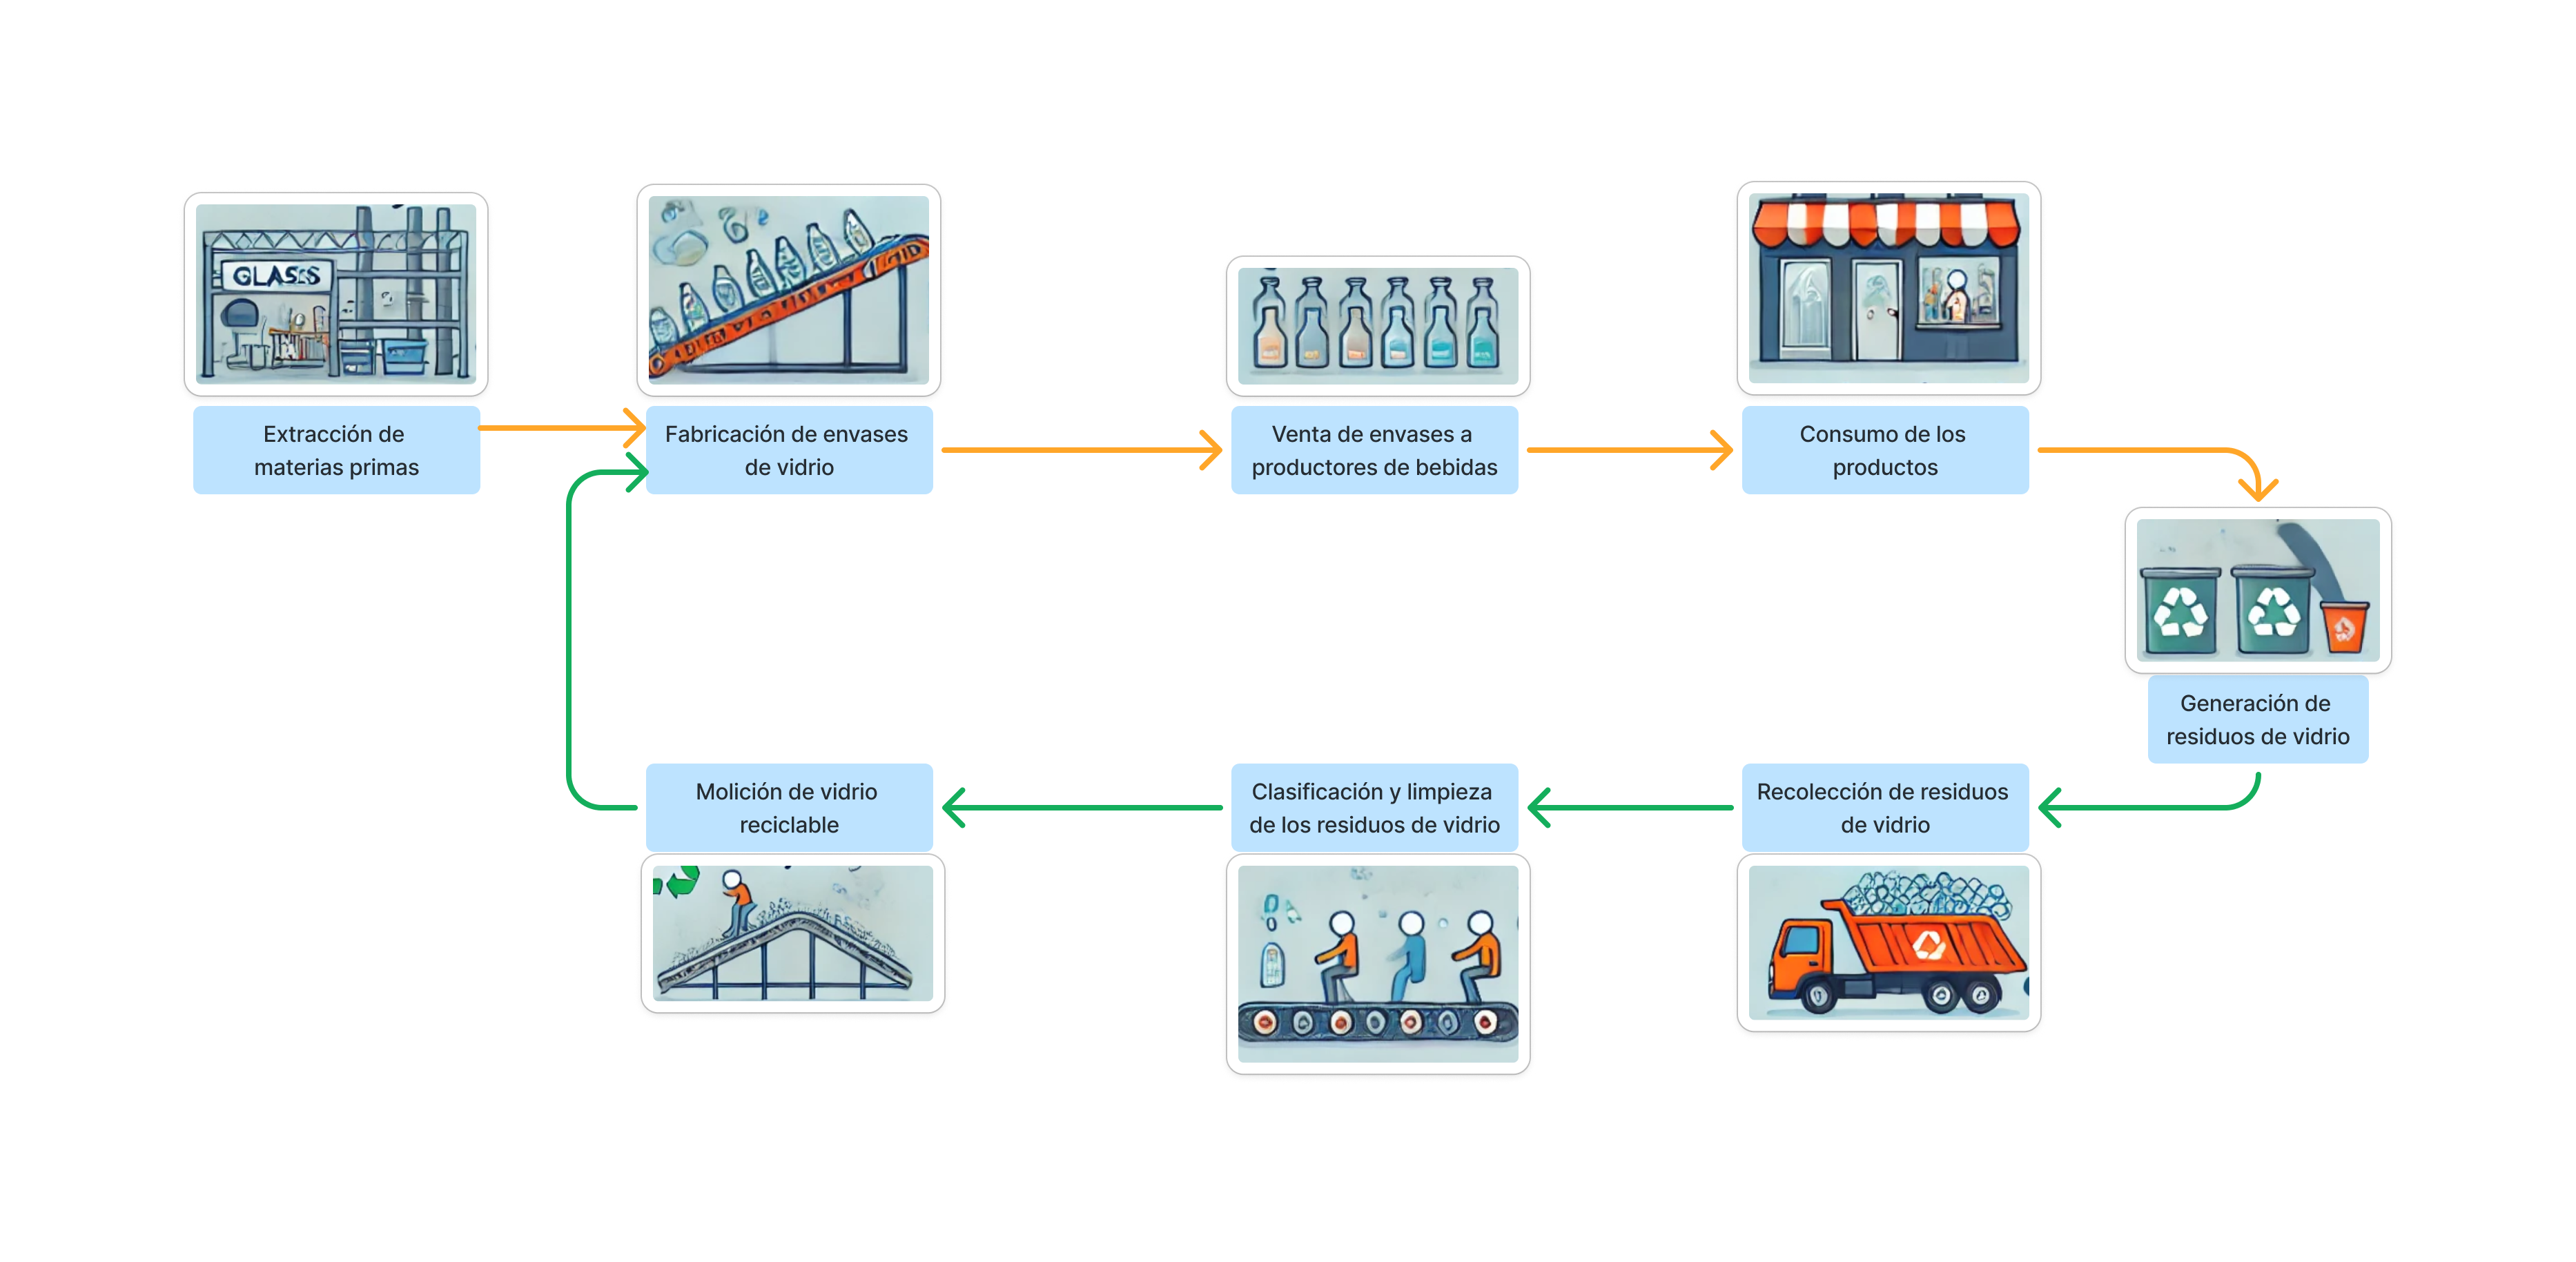
\includegraphics[width=0.6\textwidth]{Figures/glass-lifecycle.png}
    \caption{Etapas del ciclo de vida del vidrio}
    \label{fig:glass-lifecycle}
\end{figure}

En este contexto, se identifican los siguientes actores clave:
\begin{itemize}
		\item **Productor de Vidrio:** Encargado de la fabricación del vidrio, quien debe registrar la información del lote producido.
		\item **Productor de Alimentos Embotellados:** Utiliza el vidrio para envasar productos, y debe poder acceder a la trazabilidad del vidrio utilizado.
		\item **Consumidor:** Usuario final que adquiere productos envasados en vidrio y puede participar en el proceso de reciclaje.
		\item **Centro de Reciclaje:** Responsable de recibir, procesar y reciclar el vidrio, asegurando que la información de trazabilidad se mantenga actualizada.
\end{itemize}

% Aclara los actores: En la lista de actores, tienes "Productor de Vidrio" y "Productor de Alimentos Embotellados". Para mayor claridad y consistencia con el ciclo de vida del vidrio, podrías considerar renombrar "Productor de Alimentos Embotellados" a algo como "Empresa Envasadora" o "Productor Secundario (usuario de envases de vidrio)".

% TODO: acá decir "en adelante, productor primario y secundario"

A partir de esta identificación, junto con la revisión de literatura, proyectos previos y entrevistas con actores del sector, se construye un \textit{Canvas de Propuesta de Valor}. Este diagrama semi-estructurado documenta de forma preliminar y flexible las necesidades y dolores de cada actor, permitiendo una comprensión más profunda de sus expectativas y requerimientos. En la Figura \ref{fig:value-proposition-canvas} se muestra el canvas elaborado para el sistema de trazabilidad de vidrio, donde se destacan por separado las necesidades y expectativas de cada actor involucrado.

\begin{figure}[!htpb]
		\centering
		\includegraphics[width=0.8\textwidth]{Figures/value-proposition-canvas.png}
		\caption{Canvas de Propuesta de Valor para el sistema de trazabilidad de vidrio}
		\label{fig:value-proposition-canvas}
\end{figure}

Con esta información, se establece un entendimiento claro de las necesidades de los actores y se sientan las bases para la siguiente fase del modelado de requerimientos, donde se definirán los casos de uso y los requerimientos funcionales y no funcionales del sistema.

\section{Modelado de Casos de Uso}
\label{sec:use-cases}

Una vez definido el dominio del problema y los actores involucrados, el siguiente paso es la identificación y modelado de los casos de uso. Los casos de uso son descripciones detalladas de cómo los actores interactúan con el sistema para lograr un objetivo específico. Cada caso de uso representa una funcionalidad del sistema desde la perspectiva del usuario.

En el caso de un prototipo de sistema de trazabilidad de vidrio, los casos de uso pueden incluir acciones como el registro de un nuevo lote de vidrio por parte del productor, la consulta de la trazabilidad del vidrio por parte del consumidor, o el registro de la recepción de un lote por parte del centro de reciclaje. A su vez, dado que es un prototipo tecnológico, se deben incluir casos de uso relacionados con la interacción del usuario con la plataforma, como la autenticación de usuarios y la visualización de datos en la interfaz.

Los casos de uso se pueden representar gráficamente mediante diagramas de casos de uso, que muestran las interacciones entre los actores y el sistema. En la Figura \ref{fig:use-case-diagram} se presenta un diagrama de casos de uso para el sistema de trazabilidad de vidrio, donde se ilustran las principales funcionalidades y los actores involucrados. Cada caso de uso está asociado a un actor específico, lo que permite visualizar claramente las interacciones y responsabilidades de cada uno. En caso de que un caso de uso se comparta entre varios actores, se puede representar como un caso de uso heredado, lo que indica que varios actores pueden realizar la misma acción o funcionalidad. % Explicar bien lo de la herencia o mencionar como se ve en el diagrama.

\begin{figure}[!htpb]
		\centering
		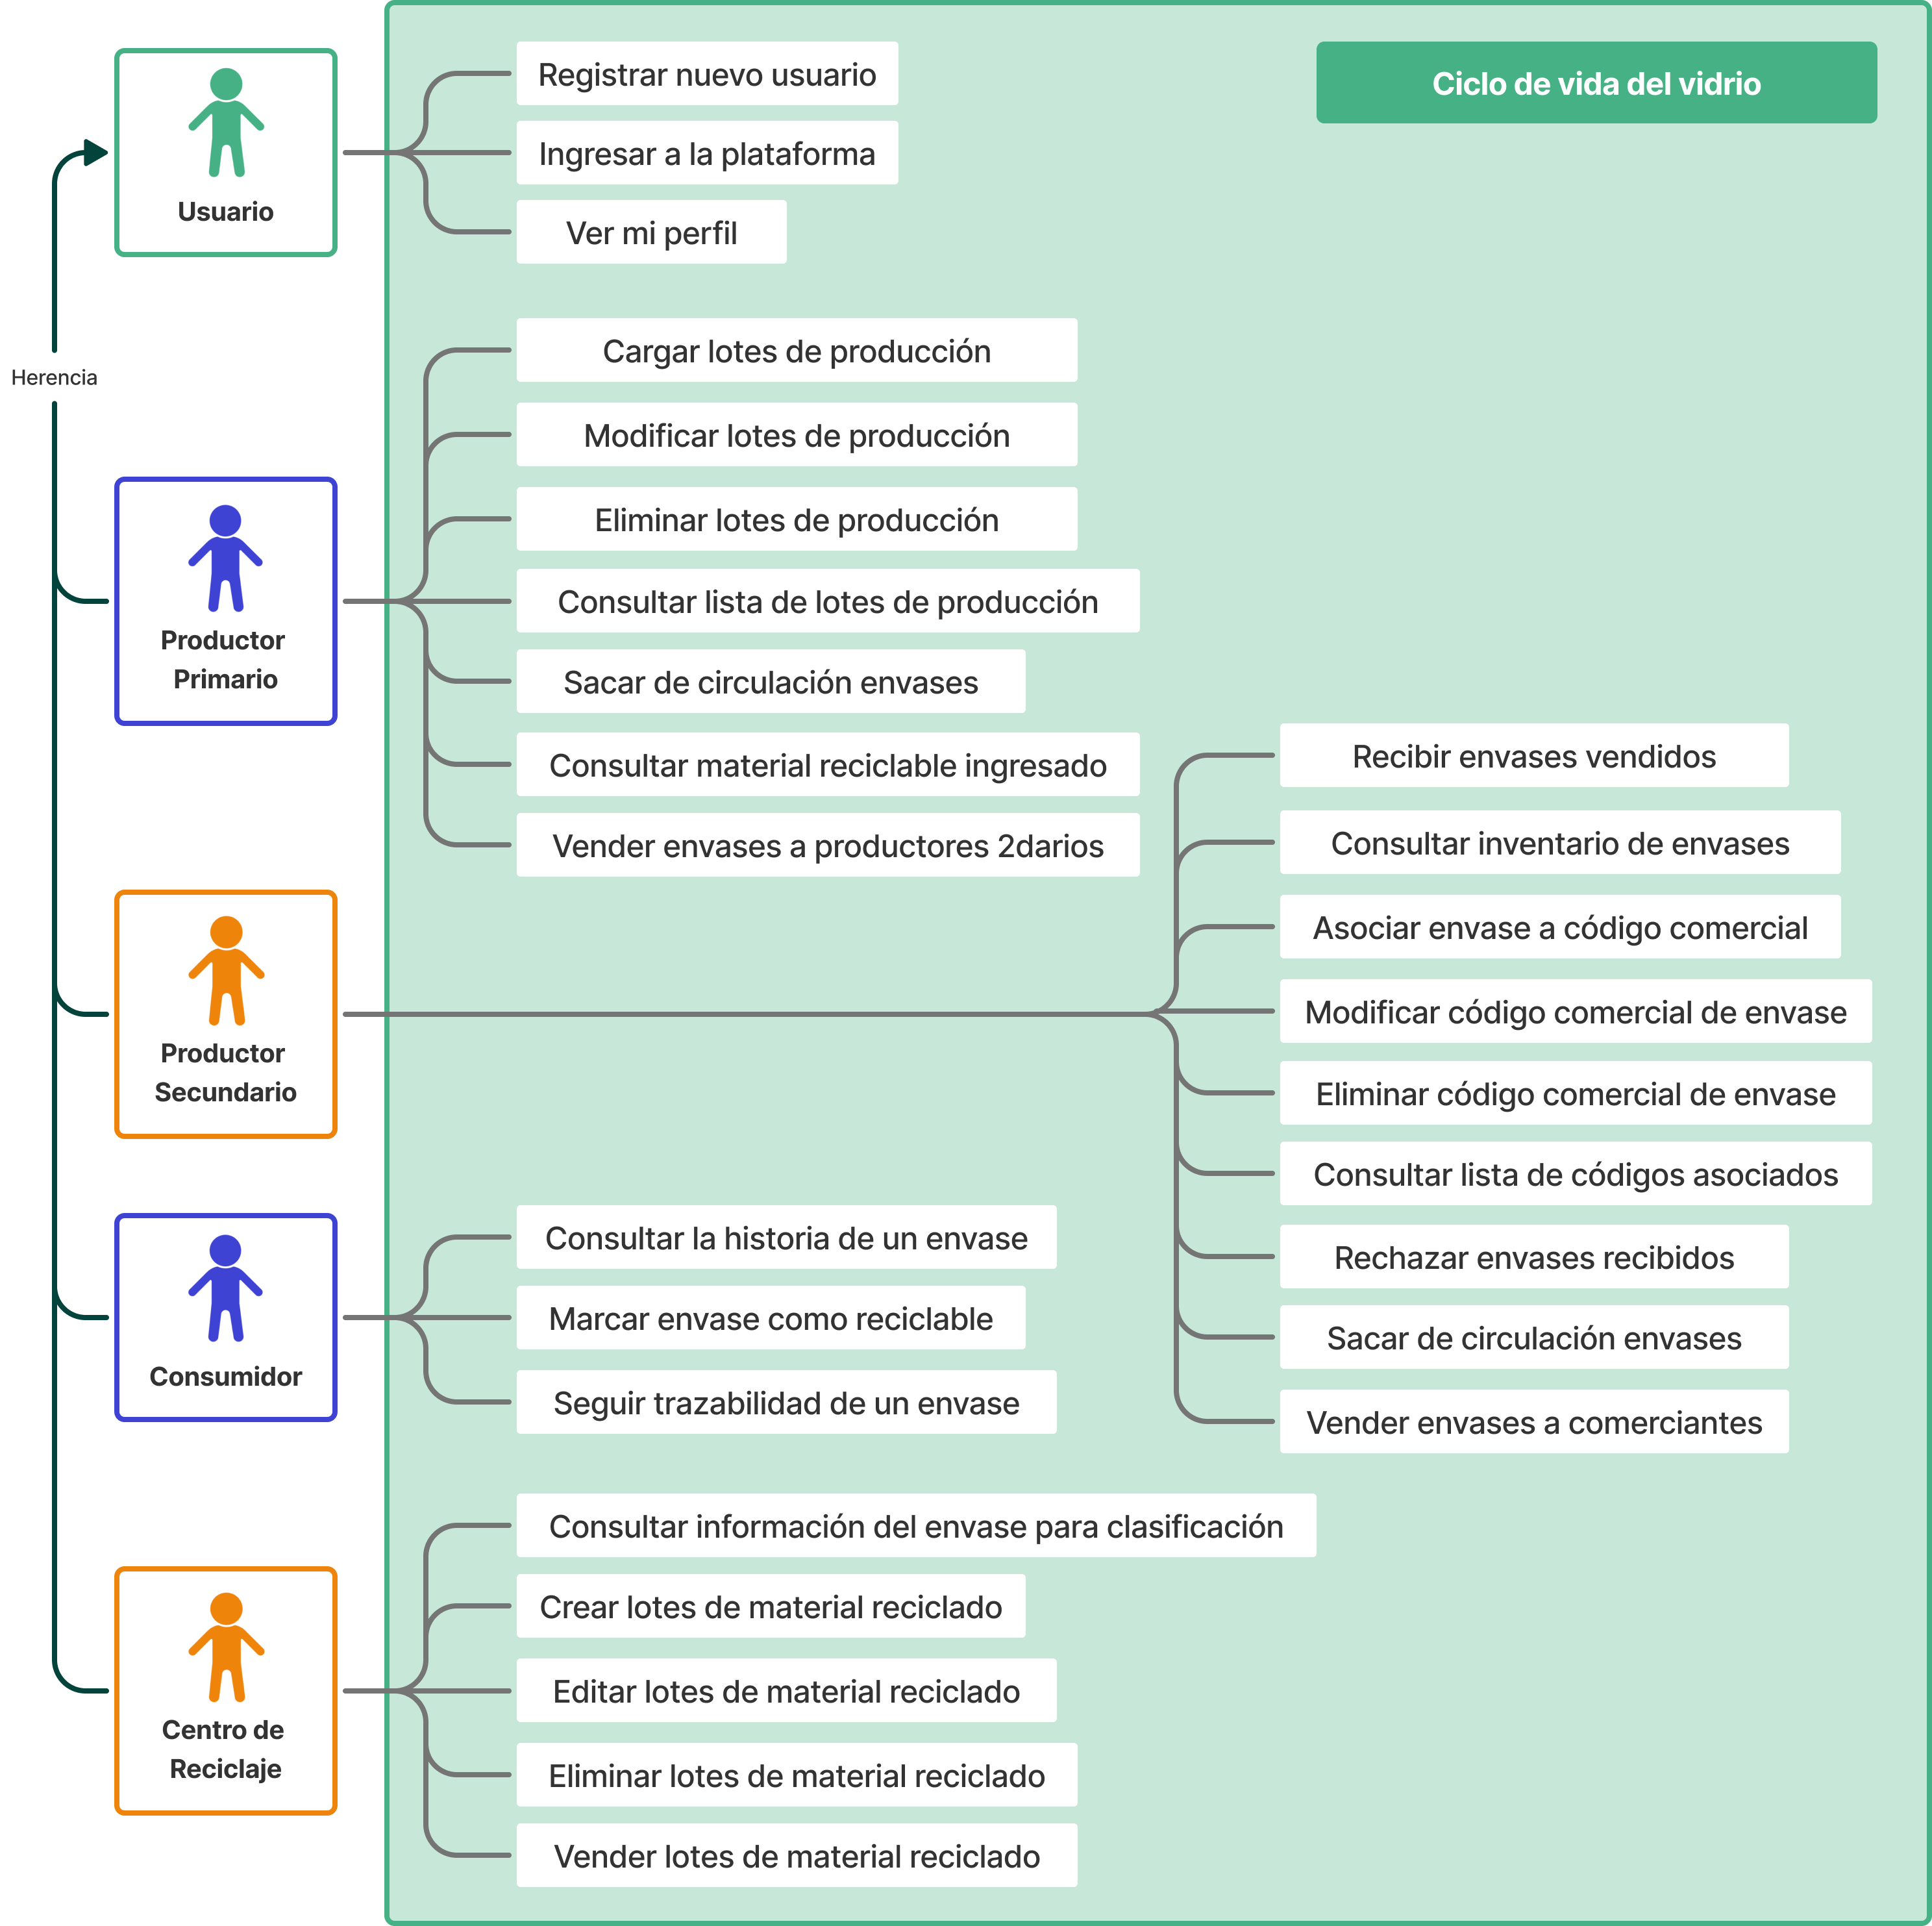
\includegraphics[width=0.8\textwidth]{Figures/use-case-diagram.png}
		\caption{Diagrama de Casos de Uso del sistema de trazabilidad de vidrio}
		\label{fig:use-case-diagram}
\end{figure}

En el diagrama de casos de uso se puede observar que cada actor tiene un conjunto de casos de uso asociados, relacionados con sus responsabilidades y acciones dentro del sistema. Por ejemplo, el Productor de Vidrio tiene casos de uso para registrar un nuevo lote de vidrio, consultar la trazabilidad de un lote específico y actualizar la información del lote. El Centro de Reciclaje, por su parte, tiene casos de uso para recibir lotes de vidrio, registrar el reciclaje y consultar la trazabilidad de los lotes recibidos. Al tratarse de un sistema de trazabilidad para economía circular, los casos de uso de cada actor están interrelacionados de forma cíclica, lo que permite una trazabilidad completa del vidrio a lo largo de su ciclo de vida. Por ejemplo, el caso de uso "Vender envases a productores 2darios" del Productor de Vidrio está relacionado con los casos de uso "Recibir envases vendidos" y "Rechazar envases recibidos" del Productor de Bebidas Envasadas, lo que permite rastrear el vidrio desde su producción hasta su reciclaje y reutilización.

A partir de este listado de casos de uso, se procede a la definición de los requerimientos funcionales y no funcionales del sistema. Cada caso de uso se descompone en requerimientos específicos que describen las funcionalidades que el sistema debe implementar para cumplir con las expectativas de los actores.

\section{Definición de Requerimientos}
\label{sec:requirements-definition}

Una vez identificados los casos de uso, el siguiente paso es la definición de los requerimientos funcionales y no funcionales del sistema. Los requerimientos funcionales describen las funcionalidades específicas que el sistema debe proporcionar, mientras que los no funcionales establecen las características de calidad que el sistema debe cumplir, como rendimiento, seguridad, usabilidad, entre otros.

Los requerimientos se documentan de manera estructurada, asignando un identificador único a cada uno para facilitar su seguimiento y gestión. Cada requerimiento se describe de forma clara y concisa, especificando su propósito, las condiciones bajo las cuales debe cumplirse y las dependencias con otros requerimientos. Por ejemplo, un requerimiento funcional podría ser: "El sistema debe permitir al Productor de Vidrio registrar un nuevo lote de vidrio, especificando la cantidad y el tipo de vidrio". Un requerimiento no funcional podría ser: "El sistema debe garantizar la seguridad de los datos del usuario mediante autenticación y autorización adecuadas".

En este trabajo, se han identificado un total de XX requerimientos funcionales y YY requerimientos no funcionales a partir de los casos de uso definidos. Estos requerimientos se han documentado en un formato que permite su fácil comprensión y seguimiento durante el desarrollo del sistema. Además, se han establecido dependencias entre los requerimientos, lo que permite identificar cuáles son necesarios para implementar otros. Por ejemplo, el requerimiento de registrar un lote de vidrio (RF-01) es una dependencia para el requerimiento de recibir un lote en el centro de reciclaje (RF-02). En la Tabla \ref{tab:functional-requirements} se presenta la lista de requerimientos funcionales identificados, junto con sus descripciones y dependencias. En la Tabla \ref{tab:non-functional-requirements} se muestra la lista de requerimientos no funcionales identificados para el sistema.

\begin{table}[!htpb]
		\centering
		\caption{Requerimientos Funcionales del sistema de trazabilidad de vidrio}
		\label{tab:functional-requirements}
		\begin{tabular}{|c|p{8cm}|p{4cm}|}
				\hline
				\textbf{ID} & \textbf{Descripción} & \textbf{Dependencias} \\
				\hline
				RF-01 & El sistema debe permitir al Productor de Vidrio registrar un nuevo lote de vidrio, especificando la cantidad y el tipo de vidrio. & - \\
				RF-02 & El sistema debe permitir al Centro de Reciclaje recibir un lote de vidrio, validando la información del lote registrado. & RF-01 \\
				RF-03 & El sistema debe permitir al Consumidor consultar la trazabilidad de un lote de vidrio específico. & RF-01, RF-02 \\
				% Agregar más requerimientos según sea necesario
				\hline
		\end{tabular}
\end{table}

\begin{table}[!htpb]
		\centering
		\caption{Requerimientos No Funcionales del sistema de trazabilidad de vidrio}
		\label{tab:non-functional-requirements}
		\begin{tabular}{|c|p{8cm}|}
				\hline
				\textbf{ID} & \textbf{Descripción} \\
				\hline
				RNF-01 & El sistema debe garantizar la seguridad de los datos del usuario mediante autenticación y autorización adecuadas. \\
				RNF-02 & El sistema debe asegurar la inmutabilidad de los datos registrados en la blockchain. \\
				RNF-03 & El sistema debe proporcionar un rendimiento aceptable en la ejecución de transacciones, con un tiempo de respuesta máximo de 2 segundos. \\
				% Agregar más requerimientos no funcionales según sea necesario
				\hline
		\end{tabular}
\end{table}

Con esta lista de requerimientos, se establece una base sólida para la siguiente fase del modelado de requerimientos, donde se definirán las historias de usuario y se planificará el desarrollo del sistema.
\section{Historias de Usuario y Planificación}
\label{sec:user-stories}

Una vez definidos los requerimientos funcionales y no funcionales, el siguiente paso es la creación de historias de usuario. Las historias de usuario son descripciones breves y concisas de una funcionalidad desde la perspectiva del usuario final. Siguiendo el formato "Como [rol], quiero [acción], para [beneficio]", las historias de usuario permiten comprender mejor las necesidades del usuario y priorizar las funcionalidades a implementar.

Cada historia de usuario se asocia a uno o más requerimientos funcionales y no funcionales, y se complementa con criterios de aceptación que definen las condiciones que deben cumplirse para considerar la historia como completada. Estos criterios guían el desarrollo y las pruebas, asegurando que la funcionalidad implementada cumpla con las expectativas del usuario.

En la Tabla \ref{tab:user-stories} se presenta un ejemplo de historias de usuario para el sistema de trazabilidad de vidrio, junto con sus criterios de aceptación. Cada historia de usuario está vinculada a los requerimientos previamente definidos, lo que permite una trazabilidad clara entre los requerimientos y las funcionalidades a implementar.

\begin{table}[!htpb]
	\centering
	\caption{Historias de Usuario del sistema de trazabilidad de vidrio}
	\label{tab:user-stories}
	\begin{tabular}{|c|p{8cm}|p{4cm}|}
		\hline
		\textbf{ID} & \textbf{Historia de Usuario} & \textbf{Criterios de Aceptación} \\
		\hline
		U-01 & Como Productor de Vidrio, quiero registrar un nuevo lote de vidrio, para que pueda ser reciclado. & - El lote se registra correctamente en el sistema. \\
		U-02 & Como Centro de Reciclaje, quiero recibir un lote de vidrio, para asegurarme de que cumple con los estándares. & - El sistema valida la información del lote. \\
		U-03 & Como Consumidor, quiero consultar la trazabilidad de un lote de vidrio, para conocer su historia. & - Se muestra la información de trazabilidad del lote. \\
		% Agregar más historias de usuario según sea necesario
		\hline
	\end{tabular}
\end{table}

Las historias de usuario se redactan desde la perspectiva de los diferentes actores del sistema, lo que permite una comprensión más clara de sus necesidades y expectativas. Esta etapa, en el contexto del modelo en V, se correlaciona con la fase de pruebas de aceptación del lado derecho. Esto significa que los requerimientos que se documentan en esta fase serán la base para crear los casos de prueba que se utilizarán al final del proyecto, para verificar si el sistema cumple con lo que el cliente realmente pidió. De modo que las historias de usuario no solo guían el desarrollo, sino que también establecen los criterios para las pruebas de aceptación.

En este trabajo de tesis, se han definido un total de XX historias de usuario que abarcan todos los requerimientos funcionales y no funcionales identificados. Estas historias de usuario se han registrado en la herramienta Jira, donde se gestionarán durante el desarrollo del sistema. En Jira, cada historia de usuario se asigna a un miembro del equipo, se estima su esfuerzo y se planifica su implementación en iteraciones o sprints. Al realizar una estimación de esfuerzo, se considera la complejidad técnica, el tiempo requerido y las dependencias con otras historias de usuario. Esto permite una planificación realista del desarrollo. En la Figura \ref{fig:jira-board} se muestra un ejemplo del tablero de Jira donde se gestionan las historias de usuario, permitiendo una visualización clara del estado de cada historia y su progreso a lo largo del desarrollo. Mientras que en la Figura \ref{fig:gantt-chart} se presenta un diagrama de Gantt preliminar que ilustra la planificación del proyecto, mostrando las historias de usuario, sus dependencias y los plazos estimados para su implementación. Se puede observar en el diagrama que con la planificación armada, se estima la duración del proyecto en XX semanas, con un total de YY historias de usuario a implementar.

\begin{figure}[!htpb]
	\centering
	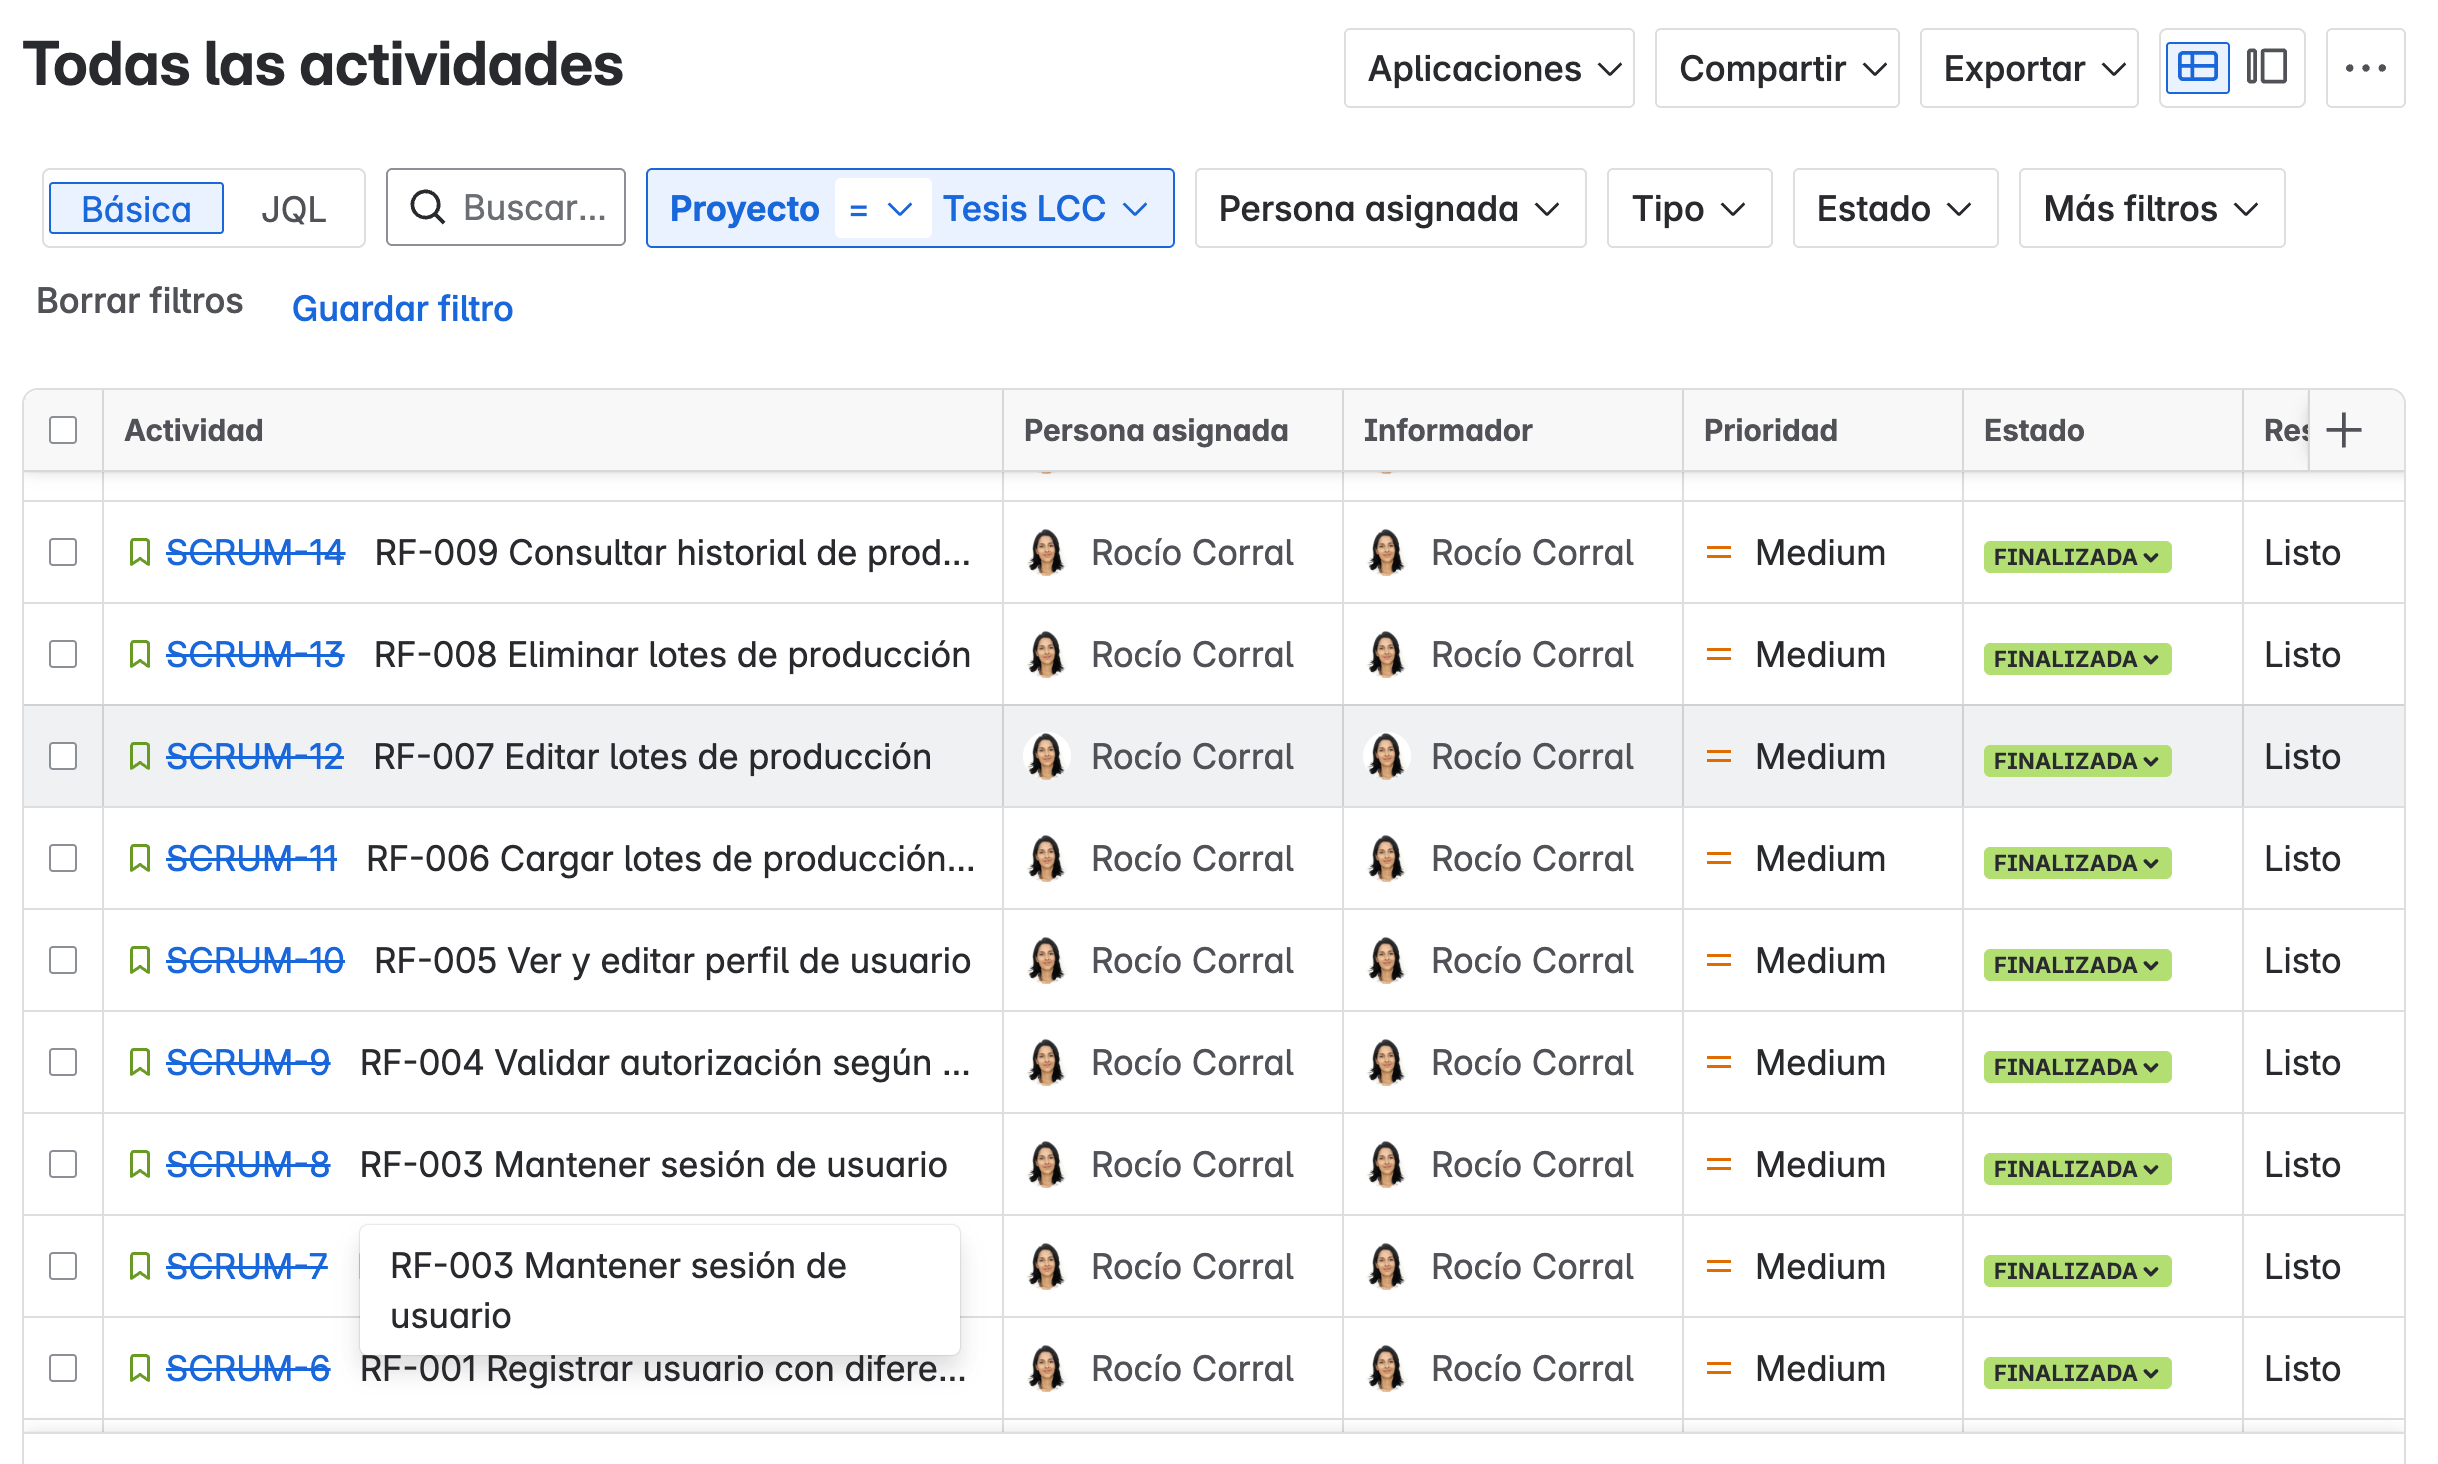
\includegraphics[width=0.8\textwidth]{Figures/jira-board.png}
	\caption{Tablero de Jira para la gestión de historias de usuario}
	\label{fig:jira-board}
\end{figure}

\begin{figure}[!htpb]
	\centering
	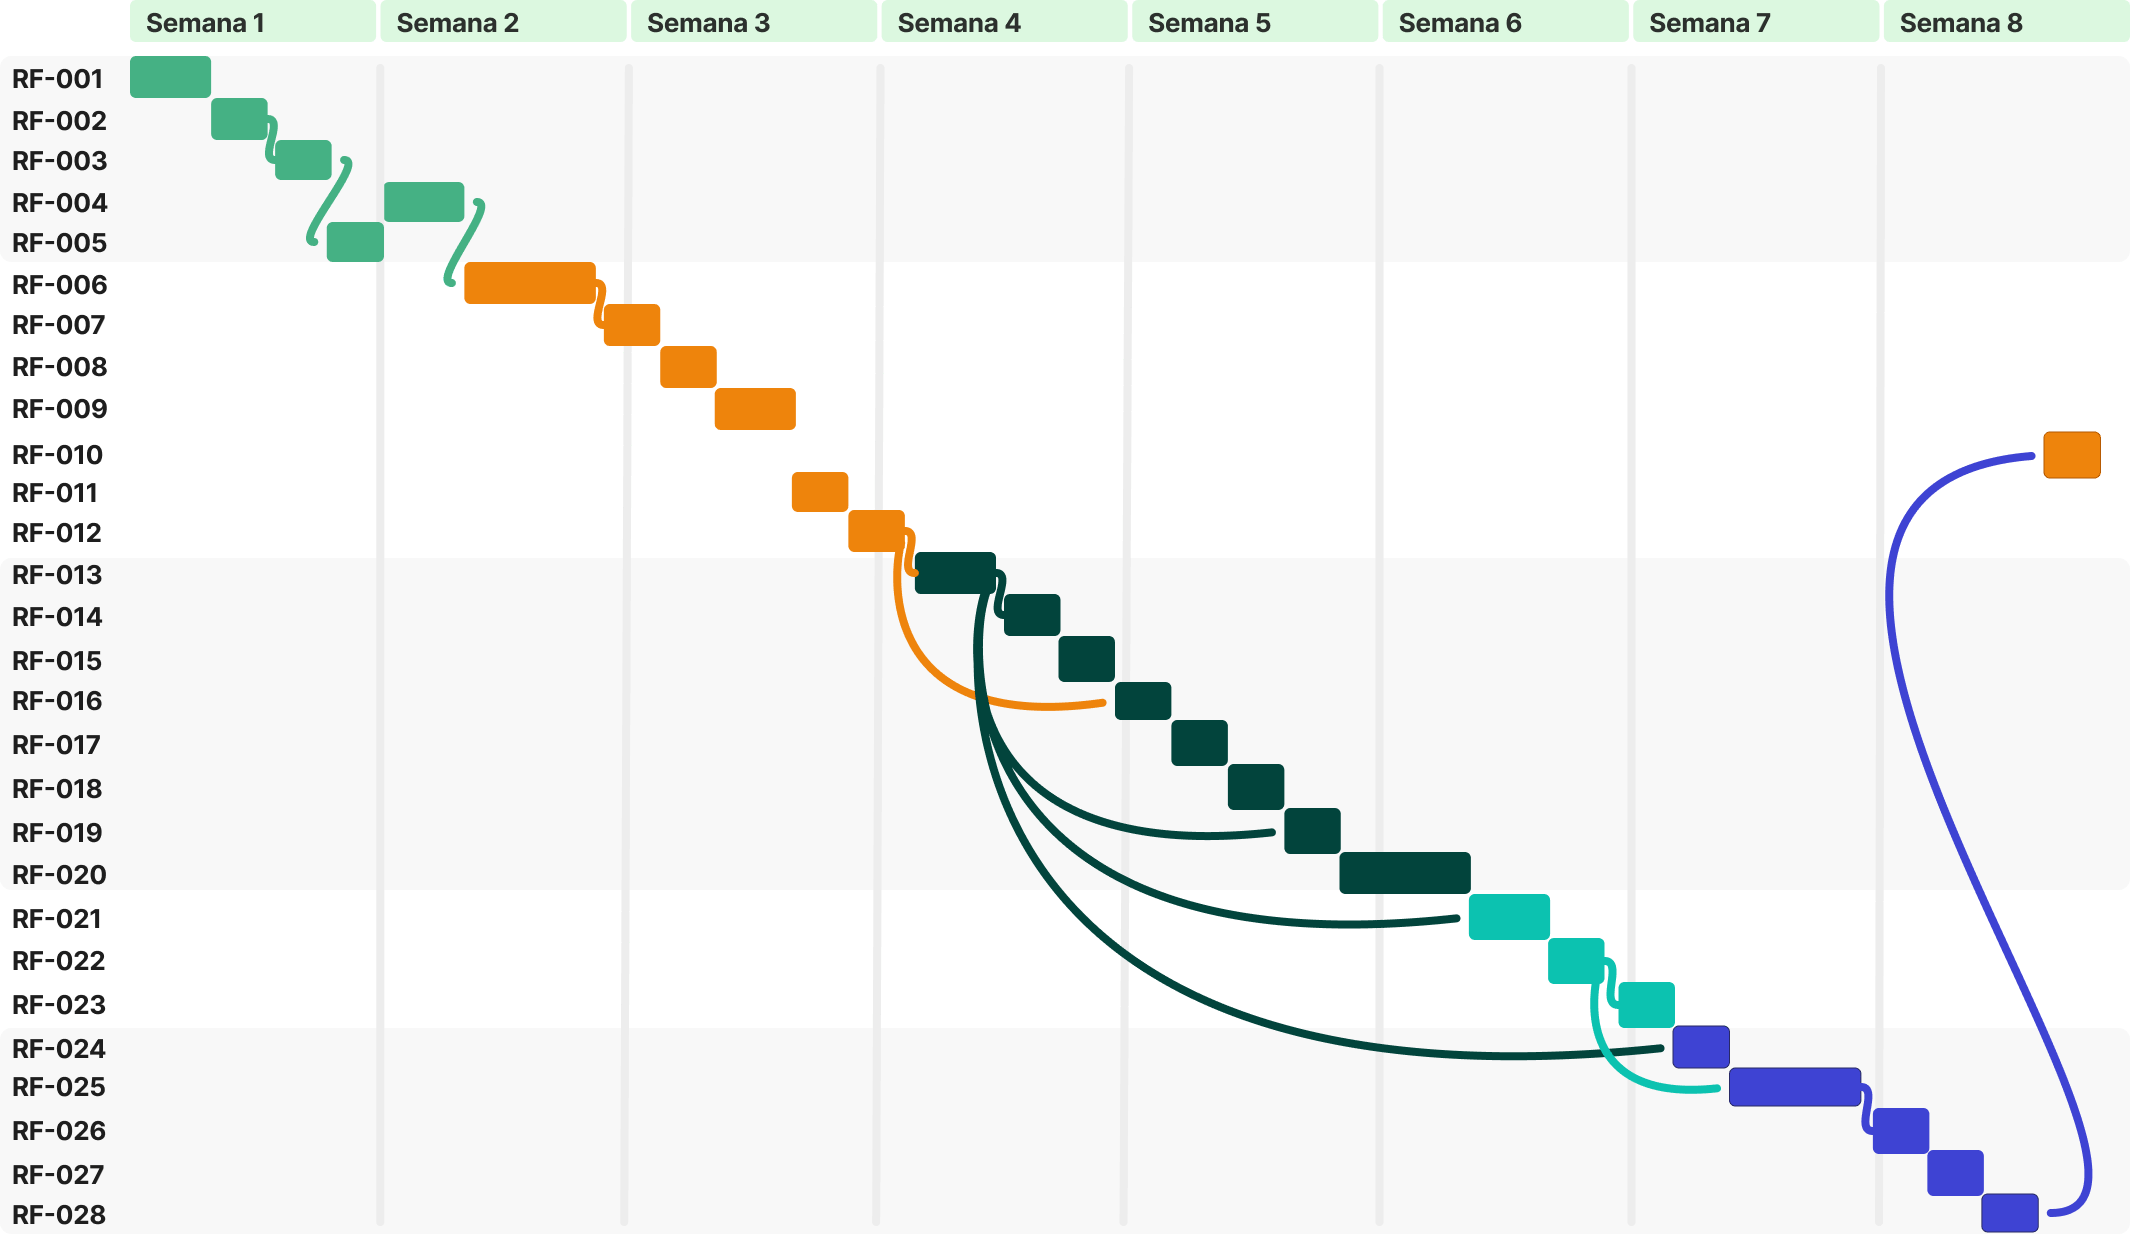
\includegraphics[width=0.8\textwidth]{Figures/gantt-chart.png}
	\caption{Diagrama de Gantt para la planificación del proyecto}
	\label{fig:gantt-chart}
\end{figure}

Con esta planificación, se establece un marco claro para el desarrollo del sistema de trazabilidad de vidrio, asegurando que todas las funcionalidades necesarias estén contempladas y que se puedan implementar de manera ordenada y eficiente. Además, se garantiza que los requerimientos funcionales y no funcionales estén alineados con las expectativas de los actores involucrados, lo que contribuye al éxito del proyecto. En el próximo capítulo, se abordará la fase de diseño de arquitectura y componentes del sistema, donde se definirán las soluciones tecnológicas y la estructura del software para cumplir con los requerimientos establecidos.

-----------------

En esta sección cuento cómo arrancamos, cuáles fueron los pasos para conseguir información y a partir de qué datos modelamos los requerimientos y cómo. Cómo bajamos los requerimientos funcionales y no funcionales, y cómo los pulimos e iteramos. Cómo despriorizamos algunos requerimientos y por qué durante este proceso.

Cómo bajamos a jira estos requerimientos y armamos una planificación tentativa del desarrollo de estas funcionalidades.

Contar que estos requerimientos se usan para realizar el diseño de la solución de software.

-----------

### **Modelado de Requerimientos**

En esta primera fase del ciclo de vida del proyecto, se identificaron y documentaron los requerimientos funcionales y no funcionales de la aplicación de trazabilidad. El objetivo principal fue comprender las necesidades del sistema desde la perspectiva de los diferentes actores (productores, centros de reciclaje, consumidores) para asegurar que el producto final cumpliera con los objetivos de la tesis: garantizar una trazabilidad transparente y la valorización del vidrio.

El proceso se llevó a cabo siguiendo una secuencia lógica:

1.  **Análisis del dominio del problema:** Se revisaron las etapas del ciclo de vida del vidrio y los puntos clave donde la trazabilidad sería crítica para la valorización.
2.  **Identificación de actores:** Se definieron los roles que interactuarían con el sistema, tales como **Productor de Vidrio**, **Centro de Reciclaje**, **Consumidor** y **Administrador del Sistema**.

---

### **Definición de Casos de Uso**

A partir del análisis de los actores y del dominio del problema, se elaboró un conjunto de **casos de uso** para describir las interacciones del sistema. Un caso de uso describe una secuencia de acciones que el sistema realiza para producir un resultado observable y de valor para un actor específico.

Para cada caso de uso, se definió:

* **Actor principal:** El usuario que inicia la acción.
* **Precondiciones:** El estado que debe tener el sistema antes de que el caso de uso pueda ejecutarse.
* **Flujo normal:** Los pasos esperados para lograr el objetivo.
* **Flujos alternativos:** Pasos que pueden ocurrir bajo diferentes circunstancias.
* **Postcondiciones:** El estado final del sistema después de que el caso de uso se completa con éxito.

---

### **Modelado y Detalle de Requerimientos**

Con los casos de uso definidos, se procedió a modelar los requerimientos de manera más granular. Se categorizaron los requisitos en **funcionales** y **no funcionales**. Los requerimientos funcionales detallan qué debe hacer el sistema, mientras que los no funcionales especifican cómo debe funcionar (rendimiento, seguridad, usabilidad, etc.).

* **Requerimientos Funcionales:** Se listaron detalladamente, asignando un identificador único a cada uno. Por ejemplo:
    * **RF-01:** El sistema debe permitir al **Productor de Vidrio** registrar un nuevo lote, especificando la cantidad, tipo y fecha de producción.
    * **RF-02:** El sistema debe permitir al **Centro de Reciclaje** registrar la recepción de un lote, validando la información previa.
* **Requerimientos No Funcionales:** Se identificaron requerimientos clave para el éxito del proyecto, como la **seguridad criptográfica** de las transacciones, la **inmutabilidad** de los datos registrados en la blockchain, y un **rendimiento** aceptable en la ejecución de transacciones.

Se identificaron **dependencias** entre los requerimientos. Por ejemplo, el registro de un lote (RF-01) es una dependencia para que pueda ser recibido por un centro de reciclaje (RF-02).

---

### **Historias de Usuario y Planificación**

Para la gestión ágil de las tareas, se tradujeron los requerimientos y casos de uso en **Historias de Usuario** (User Stories) en la plataforma Jira. Cada historia de usuario sigue el formato: "Como [rol], quiero [acción], para [beneficio]". Esto facilitó la comprensión y el seguimiento del trabajo para el equipo de desarrollo.

**Ejemplo de Historia de Usuario:**
> **Título:** Registrar un nuevo lote de vidrio
> **Descripción:** *Como **Productor de Vidrio**, quiero **registrar un nuevo lote de material** con su tipo y cantidad, para **iniciar el seguimiento de su ciclo de vida** en la aplicación.*
>
> **Criterios de Aceptación:**
> * Se debe poder ingresar la cantidad en kilogramos.
> * Se debe poder seleccionar el tipo de vidrio (ej., ámbar, transparente, verde).
> * La transacción debe quedar registrada en la blockchain.

Se crearon un total de **XX historias de usuario** que cubrieron todos los requerimientos funcionales y no funcionales.

Con esta información, se elaboró un **diagrama de Gantt** preliminar para la planificación del proyecto. Este diagrama visualizó la secuencia de las tareas (historias de usuario), estimando los plazos y considerando las dependencias entre ellas y la disponibilidad del equipo.

---

### **Análisis Retrospectivo y Ajustes**

Una vez finalizadas estas etapas, se realizó una retrospectiva para evaluar la precisión y completitud de los artefactos generados. Este proceso de mejora continua permitió:

* **Validar los requerimientos y casos de uso:** Se revisaron con los actores del proyecto para asegurar que no hubiera *gaps* o malentendidos.
* **Identificar cambios:** Se detectaron algunos requerimientos que necesitaban ser ajustados o detallados con mayor precisión, lo que se tradujo en la modificación de algunas historias de usuario.
* **Mejorar la planificación:** El plan inicial se ajustó para reflejar con mayor exactitud las complejidades y los tiempos de desarrollo real.

Este enfoque iterativo no solo garantizó la calidad de la etapa de modelado, sino que también demostró la flexibilidad del proceso de ingeniería de software para adaptarse a las necesidades emergentes, preparándonos para la siguiente fase del modelo en V.
